% !Mode:: "TeX:UTF-8"
\documentclass[12pt,a4paper]{article}

%%%%%%%%------------------------------------------------------------------------
%%%% 日常所用宏包

%% 控制页边距
% 如果是beamer文档类, 则不用geometry
\makeatletter
\@ifclassloaded{beamer}{}{\usepackage[top=2.5cm, bottom=2.5cm, left=2.5cm, right=2.5cm]{geometry}}
\makeatother

%% 控制项目列表
\usepackage{enumerate}

%% 多栏显示
\usepackage{multicol}

%% 算法环境
\usepackage{algorithm}  
\usepackage{algorithmic} 
\usepackage{float} 

%% 网址引用
\usepackage{url}

%% 控制矩阵行距
\renewcommand\arraystretch{1.4}

%% hyperref宏包,生成可定位点击的超链接,并且会生成pdf书签
\makeatletter
\@ifclassloaded{beamer}{
\usepackage{hyperref}
\usepackage{ragged2e} % 对齐
}{
\usepackage[%
    pdfstartview=FitH,%
    CJKbookmarks=true,%
    bookmarks=true,%
    bookmarksnumbered=true,%
    bookmarksopen=true,%
    colorlinks=true,%
    citecolor=blue,%
    linkcolor=blue,%
    anchorcolor=green,%
    urlcolor=blue%
]{hyperref}
}
\makeatother



\makeatletter % 如果是 beamer 不需要下面两个包
\@ifclassloaded{beamer}{
\mode<presentation>
{
} 
}{
%% 控制标题
\usepackage{titlesec}
%% 控制目录
\usepackage{titletoc}
}
\makeatother

%% 控制表格样式
\usepackage{booktabs}

%% 控制字体大小
\usepackage{type1cm}

%% 首行缩进,用\noindent取消某段缩进
\usepackage{indentfirst}

%%边框
\usepackage{listings}

%% 支持彩色文本、底色、文本框等
\usepackage{color,xcolor}

%% AMS LaTeX宏包: http://zzg34b.w3.c361.com/package/maths.htm#amssymb
\usepackage{amsmath,amssymb}
%% 多个图形并排
\usepackage{subfig}
%%%% 基本插图方法
%% 图形宏包
\usepackage{graphicx}
\newcommand{\red}[1]{\textcolor{red}{#1}}
\newcommand{\blue}[1]{\structure{#1}}
\newcommand{\brown}[1]{\textcolor{brown}{#1}}
\newcommand{\green}[1]{\textcolor{green}{#1}}


%%%% 基本插图方法结束

%%%% pgf/tikz绘图宏包设置
\usepackage{pgf,tikz}
\usetikzlibrary{shapes,automata,snakes,backgrounds,arrows}
\usetikzlibrary{mindmap}
%% 可以直接在latex文档中使用graphviz/dot语言,
%% 也可以用dot2tex工具将dot文件转换成tex文件再include进来
%% \usepackage[shell,pgf,outputdir={docgraphs/}]{dot2texi}
%%%% pgf/tikz设置结束


\makeatletter % 如果是 beamer 不需要下面两个包
\@ifclassloaded{beamer}{

}{
%%%% fancyhdr设置页眉页脚
%% 页眉页脚宏包
\usepackage{fancyhdr}
%% 页眉页脚风格
\pagestyle{plain}
}

%% 有时会出现\headheight too small的warning
\setlength{\headheight}{15pt}

%% 清空当前页眉页脚的默认设置
%\fancyhf{}
%%%% fancyhdr设置结束


\makeatletter % 对 beamer 要重新设置
\@ifclassloaded{beamer}{

}{
%%%% 设置listings宏包用来粘贴源代码
%% 方便粘贴源代码,部分代码高亮功能
\usepackage{listings}

%% 设置listings宏包的一些全局样式
%% 参考http://hi.baidu.com/shawpinlee/blog/item/9ec431cbae28e41cbe09e6e4.html
\lstset{
showstringspaces=false,              %% 设定是否显示代码之间的空格符号
numbers=left,                        %% 在左边显示行号
numberstyle=\tiny,                   %% 设定行号字体的大小
basicstyle=\footnotesize,                    %% 设定字体大小\tiny, \small, \Large等等
keywordstyle=\color{blue!70}, commentstyle=\color{red!50!green!50!blue!50},
                                     %% 关键字高亮
frame=shadowbox,                     %% 给代码加框
rulesepcolor=\color{red!20!green!20!blue!20},
escapechar=`,                        %% 中文逃逸字符,用于中英混排
xleftmargin=2em,xrightmargin=2em, aboveskip=1em,
breaklines,                          %% 这条命令可以让LaTeX自动将长的代码行换行排版
extendedchars=false                  %% 这一条命令可以解决代码跨页时,章节标题,页眉等汉字不显示的问题
}}
\makeatother
%%%% listings宏包设置结束


%%%% 附录设置
\makeatletter % 对 beamer 要重新设置
\@ifclassloaded{beamer}{

}{
\usepackage[title,titletoc,header]{appendix}
}
\makeatother
%%%% 附录设置结束


%%%% 日常宏包设置结束
%%%%%%%%------------------------------------------------------------------------


%%%%%%%%------------------------------------------------------------------------
%%%% 英文字体设置结束
%% 这里可以加入自己的英文字体设置
%%%%%%%%------------------------------------------------------------------------

%%%%%%%%------------------------------------------------------------------------
%%%% 设置常用字体字号,与MS Word相对应

%% 一号, 1.4倍行距
\newcommand{\yihao}{\fontsize{26pt}{36pt}\selectfont}
%% 二号, 1.25倍行距
\newcommand{\erhao}{\fontsize{22pt}{28pt}\selectfont}
%% 小二, 单倍行距
\newcommand{\xiaoer}{\fontsize{18pt}{18pt}\selectfont}
%% 三号, 1.5倍行距
\newcommand{\sanhao}{\fontsize{16pt}{24pt}\selectfont}
%% 小三, 1.5倍行距
\newcommand{\xiaosan}{\fontsize{15pt}{22pt}\selectfont}
%% 四号, 1.5倍行距
\newcommand{\sihao}{\fontsize{14pt}{21pt}\selectfont}
%% 半四, 1.5倍行距
\newcommand{\bansi}{\fontsize{13pt}{19.5pt}\selectfont}
%% 小四, 1.5倍行距
\newcommand{\xiaosi}{\fontsize{12pt}{18pt}\selectfont}
%% 大五, 单倍行距
\newcommand{\dawu}{\fontsize{11pt}{11pt}\selectfont}
%% 五号, 单倍行距
\newcommand{\wuhao}{\fontsize{10.5pt}{10.5pt}\selectfont}
%%%%%%%%------------------------------------------------------------------------


%% 设定段间距
\setlength{\parskip}{0.5\baselineskip}

%% 设定行距
\linespread{1}


%% 设定正文字体大小
% \renewcommand{\normalsize}{\sihao}

%制作水印
\RequirePackage{draftcopy}
\draftcopyName{XTUMESH}{100}
\draftcopySetGrey{0.90}
\draftcopyPageTransform{40 rotate}
\draftcopyPageX{350}
\draftcopyPageY{80}

%%%% 个性设置结束
%%%%%%%%------------------------------------------------------------------------


%%%%%%%%------------------------------------------------------------------------
%%%% bibtex设置

%% 设定参考文献显示风格
% 下面是几种常见的样式
% * plain: 按字母的顺序排列,比较次序为作者、年度和标题
% * unsrt: 样式同plain,只是按照引用的先后排序
% * alpha: 用作者名首字母+年份后两位作标号,以字母顺序排序
% * abbrv: 类似plain,将月份全拼改为缩写,更显紧凑
% * apalike: 美国心理学学会期刊样式, 引用样式 [Tailper and Zang, 2006]

\makeatletter
\@ifclassloaded{beamer}{
\bibliographystyle{apalike}
}{
\bibliographystyle{unsrt}
}
\makeatother


%%%% bibtex设置结束
%%%%%%%%------------------------------------------------------------------------

%%%%%%%%------------------------------------------------------------------------
%%%% xeCJK相关宏包

\usepackage{xltxtra,fontspec,xunicode}
\usepackage[slantfont, boldfont]{xeCJK} 

\setlength{\parindent}{2em}%中文缩进两个汉字位

%% 针对中文进行断行
\XeTeXlinebreaklocale "zh"             

%% 给予TeX断行一定自由度
\XeTeXlinebreakskip = 0pt plus 1pt minus 0.1pt

%%%% xeCJK设置结束                                       
%%%%%%%%------------------------------------------------------------------------
\usepackage{ listings} 
\usepackage{ xcolor}
%%%%%%%%------------------------------------------------------------------------
%%%% xeCJK字体设置

%% 设置中文标点样式,支持quanjiao、banjiao、kaiming等多种方式
\punctstyle{kaiming}                                        
\usepackage{framed}%%边框                                                
%% 设置缺省中文字体
%\setCJKmainfont[BoldFont={Adobe Heiti Std}, ItalicFont={Adobe Kaiti Std}]{Adobe Song Std}   
\setCJKmainfont{SimSun}
%% 设置中文无衬线字体
%\setCJKsansfont[BoldFont={Adobe Heiti Std}]{Adobe Kaiti Std}  
%% 设置等宽字体
%\setCJKmonofont{Adobe Heiti Std}                            

%% 英文衬线字体
\setmainfont{DejaVu Serif}                                  
%% 英文等宽字体
\setmonofont{DejaVu Sans Mono}                              
%% 英文无衬线字体
\setsansfont{DejaVu Sans}                                   

%% 定义新字体
\setCJKfamilyfont{song}{Adobe Song Std}                     
\setCJKfamilyfont{kai}{Adobe Kaiti Std}
\setCJKfamilyfont{hei}{Adobe Heiti Std}
\setCJKfamilyfont{fangsong}{Adobe Fangsong Std}
\setCJKfamilyfont{lisu}{LiSu}
\setCJKfamilyfont{youyuan}{YouYuan}

%% 自定义宋体
\newcommand{\song}{\CJKfamily{song}}                       
%% 自定义楷体
\newcommand{\kai}{\CJKfamily{kai}}                         
%% 自定义黑体
\newcommand{\hei}{\CJKfamily{hei}}                         
%% 自定义仿宋体
\newcommand{\fangsong}{\CJKfamily{fangsong}}               
%% 自定义隶书
\newcommand{\lisu}{\CJKfamily{lisu}}                       
%% 自定义幼圆
\newcommand{\youyuan}{\CJKfamily{youyuan}}                 

%%%% xeCJK字体设置结束
%%%%%%%%------------------------------------------------------------------------

%%%%%%%%------------------------------------------------------------------------
%%%% 一些关于中文文档的重定义
\newcommand{\chntoday}{\number\year\,年\,\number\month\,月\,\number\day\,日}
%% 数学公式定理的重定义

%% 中文破折号,据说来自清华模板
\newcommand{\pozhehao}{\kern0.3ex\rule[0.8ex]{2em}{0.1ex}\kern0.3ex}

\newtheorem{example}{例}                                   
\newtheorem{theorem}{定理}[section]                         
\newtheorem{definition}{定义}
\newtheorem{axiom}{公理}
\newtheorem{property}{性质}
\newtheorem{proposition}{命题}
\newtheorem{lemma}{引理}
\newtheorem{corollary}{推论}
\newtheorem{remark}{注解}
\newtheorem{condition}{条件}
\newtheorem{conclusion}{结论}
\newtheorem{assumption}{假设}

\makeatletter %
\@ifclassloaded{beamer}{

}{
%% 章节等名称重定义
\renewcommand{\contentsname}{目录}     
\renewcommand{\indexname}{索引}
\renewcommand{\listfigurename}{插图目录}
\renewcommand{\listtablename}{表格目录}
\renewcommand{\appendixname}{附录}
\renewcommand{\appendixpagename}{附录}
\renewcommand{\appendixtocname}{附录}
%% 设置chapter、section与subsection的格式
\titleformat{\chapter}{\centering\huge}{第\thechapter{}章}{1em}{\textbf}
\titleformat{\section}{\centering\sihao}{\thesection}{1em}{\textbf}
\titleformat{\subsection}{\xiaosi}{\thesubsection}{1em}{\textbf}
\titleformat{\subsubsection}{\xiaosi}{\thesubsubsection}{1em}{\textbf}

\@ifclassloaded{book}{

}{
\renewcommand{\abstractname}{摘要}
}
}
\makeatother

\renewcommand{\figurename}{图}
\renewcommand{\tablename}{表}

\makeatletter
\@ifclassloaded{book}{
\renewcommand{\bibname}{参考文献}
}{
\renewcommand{\refname}{参考文献} 
}
\makeatother

\floatname{algorithm}{算法}
\renewcommand{\algorithmicrequire}{\textbf{输入:}}
\renewcommand{\algorithmicensure}{\textbf{输出:}}

%%%% 中文重定义结束
%%%%%%%%------------------------------------------------------------------------

%\linespread{1.5}
\usepackage{parskip}%首行缩进
\setlength{\parindent}{0cm}%首行缩进

\title{}
\author{作者}
\date{\chntoday}
\begin{document}
\maketitle
\newpage
\subsection*{\color{blue}第六讲\qquad 线性方程组的迭代解法}
\subsubsection*{\color{blue}1\quad 离散Poisson方程}
\subsubsection*{\color{blue}2\quad 定常迭代算法}
\subsubsection*{\color{blue}3\quad 收敛性分析}
\subsubsection*{\color{blue}4\quad 加速算法}
\subsubsection*{\color{blue}5\quad 交替方向与HSS算法}
\subsubsection*{\color{blue}6\quad 快速Poisson算法}
方法综述\\
\begin {itemize}
	\item 直接法\quad PLU分解, LDLT分解, Cholesky分解法\\
        \item 迭代法\\
                -经典(定常,不动点)迭代法:Jacobi/Gauss-Seidel, SOR, AOR等\\
        \item -Krylov子空间迭代法: CG, MIRES, GMRES, BiCGStab等\\
        \item 快速算法\\
		-基于快速变换,如FFT, DCT, DST等\\
                -代数多重网格法(Algebraic multigrid)\\
                -快速多极子算法(Fast multipole)\\
\end{itemize}
有些方法可能只是对某类方程有效,如快速算法.在实际应用中,这些方法可以结合使用,如混合(hybrid)算法,预处理算法(preconditioning)等\\
\centerline{本讲主要介绍定常迭代算法}
更多迭代方法可参见{\color{blue}Templates for the Solution of Linear Systems:Building Blocks for Iterative Methods,}SLAM,1994\\
\section{\color{blue} 离散Poisson方程}
\subsection*{\color{blue}1.1\quad 一维Poisson方程}
\subsection*{\color{blue}1.2\quad 二维Poisson方程}
在本讲中,我们以一个典型的线性方程组为例,逐个介绍各种迭代方法,并比较它们之间的性能.这个方程组就是二维Poisson方程经过五点差分离散后得到的线性方程组.\\
\subsection{\color{blue}一维Poisson方程}
考虑如下带Dirichlet边界条件的一维Poisson方程
\begin{align}
	\begin{cases}
		\frac{\mathrm{d^2} u(x)}{\mathrm{d}x^2} =f(x),0<x<1,\\
		u(0)=a,u(1) = b\\
	\end{cases}
	\tag{6.1}
\end{align}
其中$f(x)$是给定的函数,$u(x)$是需要计算的未知函数.\\
 差分离散\\
取步长$h=\frac{1}{n+1}$,为节点$x_i=ih,i=0,1,2,...,n+1$我们采用中心差分离散,可得$(i=1,2,...,n)$
$$
-\left.\frac{d^{2} u(x)}{d x^{2}}\right|_{x_{i}}=\frac{2 u\left(x_{i}\right)-u\left(x_{i-1}\right)-u\left(x_{i+1}\right)}{h^{2}}+O\left(h^{2} \cdot\left\|\frac{d^{4} u}{d x^{4}}\right\|_{\infty}\right)
$$
将其代入(6.1),舍去高阶项后可得Poisson方程在$x_i$点的近似离散方程
$$\boxed{-u_{i-1}+2u_i-u_{i+1}=h^2f_i,}$$
其中$fi=f(xi),ui$为$u(xi)$的近似.\\
令$i= 1,2,...,n,$则可0得$n$个线性方程,写成矩阵形式
\begin{align}
	{T_nu=f,}
	\tag{6.2}
\end{align}
其中
\begin{equation}
	T_{n}=\left[\begin{array}{cccc}{2} & {-1} & {} & {} \\ {-1} & {\ddots} & {\ddots} & {} \\ {} & {\ddots} & {\ddots} & {-1} \\ {} & {} & {-1} & {2}\end{array}\right], u=\left[\begin{array}{c}{u_{1}} \\ {u_{2}} \\ {\vdots} \\ {u_{n-1}} \\ {u_{n}}\end{array}\right], f=\left[\begin{array}{c}{f_{1}+u_{0}} \\ {f_{2}} \\ {\vdots} \\ {f_{n-1}} \\ {f_{n}+u_{n+1}}\end{array}\right]
\tag{6.3}
\end{equation}
\subsection*{ 系数矩阵$T_n$的性质}
{\color{blue}引理}\quad$T_n$的特征值和对应的特征向量分别为
$$
\lambda_k=2-2cos\frac{k\pi}{n+1},
$$
$$
z_{k}=\sqrt{\frac{2}{n+1}} \cdot\left[\sin \frac{k \pi}{n+1}, \sin \frac{2 k \pi}{n+1}, \ldots, \sin \frac{n k \pi}{n+1}\right]^{T}
$$

即$Tn=ZAZ_T$,其中$A=diag(\lambda_1,\lambda_2,...,\lambda_n),Z= [z_1,z_2,...,z_n].$\\
{\color{blue}证明}.直接带入验证即可.\\
{\color{blue}引理}\quad 更一般的,设$T=tridiag(a,b,c)\in \mathbb{R}^{n\times n}$,则T的特征值为
$$
\lambda_k=b-2\sqrt{ac}cos\frac{k\pi}{n+1},k=1,2,...,n
$$
对应的特征向量为$z_k$,其第j个分量为
$$
z_k(j)=(\frac{a}{c})^{\frac{j}{2}}sin\frac{jk\pi}{n+1}
$$
特别地,若$a=c=1$,则对应的单位特征向量为
$$
z_{k}=\sqrt{\frac{2}{n+1}} \cdot\left[\sin \frac{k \pi}{n+1}, \sin \frac{2 k \pi}{n+1}, \ldots, \sin \frac{n k \pi}{n+1}\right]^{T}
$$
由前面的结论可知,$T_n$是对称正定的,其最大特征值为
$$
2\left(1-\cos \frac{n \pi}{n+1}\right)=4 \sin ^{2} \frac{n \pi}{2(n+1)} \approx 4,
$$
最小特征值为
$$
2\left(1-\cos \frac{\pi}{n+1}\right)=4 \sin ^{2} \frac{\pi}{2(n+1)} \approx\left(\frac{\pi}{n+1}\right)^{2}
$$
因此,当n很大时,$T_n$的谱条件数约为
$$
\kappa_{2}\left(T_{n}\right) \approx \frac{4(n+1)^{2}}{\pi^{2}}
$$
矩阵$T_n$可以分解为T$_n=DD^T$,其中
$$
D=\left[\begin{array}{ccccc}{-1} & {1} & {} & {} & {} \\ {} & {-1} & {1} & {} \\ {} & {} & {\ddots} & {\ddots} \\ {} & {} & {} & {-1} & {1}\end{array}\right] \in \mathbb{R}^{n \times(n+1)}
$$
矩阵D也通常称为{\color{blue}差分矩阵}.需要注意的是,D不是方阵,因此不能用这个分解来求解线性方程组$T_nx=b.$
\subsection{\color{blue}二维Poisson方程}
\subsubsection*{现在考虑二维Poisson方程}
\begin{align}
\left\{\begin{array}{l}{-\Delta u(x, y)=-\frac{\partial^{2} u(x, y)}{\partial x^{2}}-\frac{\partial^{2} u(x, y)}{\partial y^{2}}=f(x, y), \quad(x, y) \in \Omega} \\ {u(x, y)=u_{0}(x, y), \quad(x, y) \in \partial \Omega}\end{array}\right.
\tag{6.4}
\end{align}
其中$\Omega=[0,1] \times[0,1]$为求解区域,$\partial \Omega$表示$\Omega$的边界.
\subsection*{ 五点差分离散}
为了简单起见,我们在$x-$方向和$y-$方向取相同的步长$h=\frac{1}{n+1}$,节点设为
$x_{i}=i h, y_{j}=j h, i, j=0,1,2, \ldots, n.$在$x-$方向和$y-$方向同时采用中心差分离散可得
$$
\left.\frac{\partial^{2} u(x, y)}{\partial x^{2}}\right|_{\left(x_{i}, y_{j}\right)} \approx \frac{2 u\left(x_{i}, y_{j}\right)-u\left(x_{i-1}, y_{j}\right)-u\left(x_{i+1}, y_{j}\right)}{h^{2}}
$$
$$
\left.\frac{\partial^{2} u(x, y)}{\partial y^{2}}\right|_{\left(x_{i}, y_{j}\right)} \approx \frac{2 u\left(x_{i}, y_{j}\right)-u\left(x_{i}, y_{j-1}\right)-u\left(x_{i}, y_{j+1}\right)}{h^{2}}
$$
代入({\color{blue}6.4}),即得二维Poisson方程在$(x_i, y_j)$点的近似离散方程
$$
\boxed {4 u_{i, j}-u_{i-1, j}-u_{i+1, j}-u_{i, j-1}-u_{i, j+1}=h^{2} f_{i, j}}
$$  
其中$f_{i j}=f\left(x_{i}, y_{j}\right), u_{i, j}$为$u\left(x_{i}, y_{j}\right)$的近似。
写成矩阵形式即为
\begin{align}
T_{N} u=h^{2} f
\tag{6.5}
\end{align}
其中
$$
T_{N} \triangleq I \otimes T_{n}+T_{n} \otimes I, \quad N=n^{2},
$$
$$
u=\left[u_{1,1}, \ldots, u_{n, 1}, u_{1,2}, \ldots, u_{n, 2}, \ldots, u_{1, n}, \ldots, u_{n, n}\right],
$$
在后面介绍的算法时,我们都以二维离散Poisson方程({\color{blue}6.5})为例.

\subsection*{ 系数矩阵T的性质}
因为$T_{N}=I \otimes T_{n}+T_{n} \otimes I$由Kronecker乘积的性质即得
{\color{blue}定理}\quad 设$T_{n}=Z \Lambda Z^{T}$其中$Z=\left[z_{1}, z_{2}, \ldots, z_{n}\right]$为正交阵,$\Lambda=\operatorname{diag}\left(\lambda_{1}\lambda_{2}, \dots, \lambda_{n} \right)$为对角阵,则T的特征值分解为
$$
T_{N}=(Z \otimes Z)(I \otimes \Lambda+\Lambda \otimes I)(Z \otimes Z)^{T}
$$
即T的特征值为$\lambda_{i}+\lambda_{j},$对应的特征向量为$ z_{i} \otimes z_{j}, i, j=1,2, \dots, n$
条件数
$$
\kappa\left(T_{N}\right)=\frac{\lambda_{\max }\left(T_{N}\right)}{\lambda_{\min }\left(T_{N}\right)}=\frac{1-\cos \frac{n \pi}{n+1}}{1-\cos \frac{\pi}{n+1}}=\frac{\sin ^{2} \frac{n \pi}{2(n+1)}}{\sin ^{2} \frac{\pi}{2(n+1)}} \approx \frac{4(n+1)^{2}}{\pi^{2}}
$$
故当n越来越大时$\kappa\left(T_{N}\right) \rightarrow \infty$,即$T_N$越来越病态.
\newpage
\subsection*{ 二维离散Poisson方程的常用算法}
\begin{tabular}{l|lll}
\hline
{}&方法&串行时间&存储空间\\
\hline
\hline
直接法&稠密Cholesky分解&$O(N^3)$&$O(N^2)$\\
{}&显式求逆&$O(N^2)$&$O(N^2)$\\
{}&带状Cholesky分解&$O(N^2)$&$O(N^(3/2))$\\
{}&稀疏Cholesky分解&$O(N^(3/2)))$&$O(N\log N)$\\
\hline
经典迭代&Jacobi&$O(N^3)$&$O(N)$\\
{}&Gauss-Seidel&$O(N^3)$&$O(N)$\\
{}&SOR&$O(N^(3/2)))$&$O(N)$\\
{}& 带Chebyshev加速的SSOR &$O(N^(5/4)))$&$O(N)$\\
\hline
Krylov子空间迭代&CG (共轭梯度法)&$O(N^{3/2})$&$O(N)$\\
{}&CG (带修正IC预处理)&$O(N^(5/4)))$&$O(N)$\\
\hline
快速算法&FFT(快速Fourier变换)&$O(N\log N)$&$O(N)$\\
{}&块循环约化&$O(N\log N)$&$O(N)$\\
{}&Multigrid&$O(N)$&$O(N)$\\
\hline
\end{tabular}
%\newpage
\section{\color{blue} 定常迭代方法}
%\newpage
当直接求解方程组$Ax=b$较困难时,我们可以求解一个近似方程组
$$
M x=b
$$
设其解为$x^{(1)}$.易知它与真解之间的误差满足
$$
A\left(x_{*}-x^{(1)}\right)=b-A x^{(1)}
$$
如果$x^{(1)}$已经满足精度要求,则停止计算,否则需要修正.设修正量为$\Delta x$.显然$\Delta x$满足方程$A \Delta x=b-A x^{(1)}$但由于直接求解该方程比较困难,因此我们还是求解近似
$$
M \Delta x=b-A x^{(1)}
$$
于是得到修正后的近似解
$$x^{(2)}=x^{(1)}+\Delta x=x^{(1)}+M^{-1}\left(b-A x^{(1)}\right)$$
若$x^{(2)}$已经满足精度要求,则停止计算,否则继续按以上的方式进行修正。不断重复以上步骤,于是,我们就得到一个序列
$$
x^{(1)}, x^{(2)}, \ldots, x^{(k)}, \ldots
$$
满足以下递推关系
$$
x^{(k+1)}=x^{(k)}+M^{-1}\left(b-A x^{(k)}\right), \quad k=1,2, \ldots
$$
{\color{blue}由于每次迭代的格式是一样的,因此称为\quad 定常迭代.}\\
通常,构造一个好的定常迭代,需要考虑以下两点:
\begin{itemize}
\item (1)\quad 以$M$为系数矩阵的线性方程组必须要比原线性方程组更容易求解;
\item (2)\quad $M$应该是$A$的一个很好的近似,或者迭代序列${x_k}$要收敛
\end{itemize}
下面我们就介绍几个常见的基于矩阵分裂的定常迭代方法
\begin{itemize}
\item Jacobi算法
\item Gauss-Seidel算法
\item SOR(Successive Over-Relaxation)算法
\item SSOR(Symmetric SOR)算法
\item AOR(Accelerated over-relaxation)算法
\end{itemize}
%\newpage
\subsection{\color{blue}矩阵分裂迭代方法}
迭代方法的基本思想:给定一个迭代初始值$x_{(0)}$,通过一定的迭代格式生成一个迭代序列$\left\{x^{(k)}\right\}_{k=0}^{\infty}$,使得$\lim _{k \rightarrow \infty} x^{(k)}=x_{*} \triangleq A^{-1} b$
\subsection*{定义(矩阵分裂Matrix splitting)}设$A \in \mathbb{R}^{n \times n}$非奇异,称
$$
A=M-N
$$
为$A$的一个矩阵分裂,其中$M$非奇异\\
原方程组等价于$M x=N x+b$.于是我们就可以构造出以下的迭代格式
\begin{align}
x^{(k+1)}=M^{-1} N x^{(k)}+M^{-1} b \triangleq G x^{(k)}+g \quad, \quad k=0,1, \ldots,\tag{6.7}
\end{align}


其中$G=M^{-1} N$称为该迭代格式的{\color{blue}迭代矩阵}
\subsection{\color{blue}Jacobi迭代}
将矩阵$A$分裂为$$A=D-L-U$$
其中$D$为$A$的对角部分,$-L$和$-U$分别为A的严格下三角和严格上的三角部分\\
在矩阵分裂$A=M-N$中取$M=D, N=L+U$,则可得到{\color{blue}Jacobi迭代}算法:
\begin{align}
x^{(k+1)}=D^{-1}(L+U) x^{(k)}+D^{-1} b \quad, \quad k=0,1,2, \ldots
\tag{6.8}
\end{align}
迭代矩阵为
$$
G_{1}=D^{-1}(L+U)
$$
写成分量形式即为
$$
x_{i}^{(k+1)}=\frac{1}{a_{i i}}\left(b_{i}-\sum_{j=1, j \neq i}^{n} a_{i j} x_{j}^{(k)}\right) \quad, \quad i=1,2, \ldots, n
$$
由于Jacobi迭代中$x_i^{(k+1)}$的更新顺序与$i$无关,即可以按照顺序$i=1,2,...,n$计算。因此Jacobi迭代非常适合并行计算。\\
\begin{tabular}{l}
\hline
{\color{blue}算法2.1}求解线性方程组的Jacobi迭代方法\\
\hline
1:Choose an initial guess $x^{(0)}$\\
2: while not converge do\\
3:\qquad for $i=1$ to n do\\
4:\qquad \qquad
$
x_{i}^{(k+1)}=\left(b_{i}-\sum_{j=1, j \neq i}^{n} a_{i j} x_{j}^{(k)}\right) / a_{i i}
$\\
5:\qquad end for\\
6:end while\\
\hline
\end{tabular}\\
我们也可以将Jacobi迭代格式写成\\
$$
x^{(k+1)}=x^{(k)}+D^{-1}\left(b-A x^{(k)}\right)=x^{(k)}+D^{-1} r_{k} \quad, \quad k=0,1,2, \ldots
$$
其中$r_{k} \triangleq b-A x^{(k)}$是$k$次迭代后的残量。\\
\subsection*{二维离散poisson方程Jacobi迭代方法}
\begin{tabular}{l}
\hline
{\color{blue}算法2.2}求解二维离散poisson方程的Jacobi迭代方法\\
\hline
1:Choose an initial guess $v^{(0)}$\\
2: while not converge do\\
3:\qquad for $i=1$ to $N$ do\\
4:\qquad \qquad for $j=1$ to $N$ do\\
5:\qquad \qquad \qquad
$
x_{i}^{(k+1)}=\left(b_{i}-\sum_{j=1, j \neq i}^{n} a_{i j} x_{j}^{(k)}\right) / a_{i i}
$\\
6:\qquad \qquad end for\\
7:\qquad end for\\
8:end while\\
\hline
\end{tabular}
\subsection{Gauss-Seidel迭代}
取$M=D-L,N=U$,即可得{color{blue}Gauss-Seidel (G-S)迭代}算法:
\begin{align}
x^{(k+1)}=(D-L)^{-1} U x^{(k)}+(D-L)^{-1} b\tag{6.9}
\end{align}
迭代矩阵为
$$
G_{GS}=(D-L)^{-1}U
$$
将$G-S$迭代改写为
$$
Dx^{(k+1)}=Lx^{(k+1)}+Ux^{(k)}+b
$$
即可得分量形式
$$
x_{i}^{(k+1)}=\frac{1}{a_{i i}}\left(b_{i}-\sum_{j=1}^{i-1} a_{i j} x_{j}^{(k+1)}-\sum_{j=i+1}^{n} a_{i j} x_{j}^{(k)}\right) \quad i=1,2, \ldots, n
$$
\begin{tabular}{l}
\hline
{\color{blue}算法2.1}求解线性方程组的Jacobi迭代方法\\
\hline
1:Choose an initial guess $x^{(0)}$\\
2: while not converge do\\
3:\qquad for $i=1$ to n do\\
4:\qquad \qquad
$x_{i}^{(k+1)}=\frac{1}{a_{i i}}\left(b_{i}-\sum_{j=1}^{i-1} a_{i j} x_{j}^{(k+1)}-\sum_{j=i+1}^{n} a_{i j} x_{j}^{(k)}\right)$\\
5:\qquad end for\\
6:end while\\
\hline
\end{tabular}\\
$G-S$算法的主要优点是充分利用了已经获得的最新数据。\\
但由于$G-S$算法中未知量的更新是按自然顺序进行的。因此不适合并行计算。\\
\subsection*{G-S算法的并行计算:红黑排序}

\begin{figure}[h]
\begin{minipage}[l]{0.65\linewidth} 
下面我们介绍一种适合并行计算的更新顺序:{\color{blue}红黑排序},即将二维网络点依次做红黑记号,如右图\\
在计算过程中,对未知量的值进行更新时,我们可以先更新红色节点,此时所使用的只是黑色节点的数据,然后再更新黑色节点,这时使用的是红色节点的数据.于是我们得到红黑排序G-S迭代方法.\\
\end{minipage} 
\hfill 
\begin{minipage}[t]{0.35\linewidth} 
\centering 
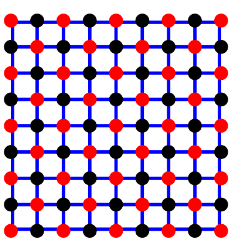
\includegraphics[width=0.8\textwidth]{./figures/figure1.png} 
\end{minipage} 
\end{figure}
\begin{tabular}{l}
\hline
{\color{blue}算法2.4}求解二维离散poisson方程的红黑排序G-S迭代方法\\
\hline
1:Choose an initial guess $v^{(0)}$\\
2: while not converge do\\
3:\qquad for $(i,j)$为红色节点 do\\
4:\qquad \qquad
$u_{i, j}^{(k+1)}=\frac{1}{4}\left(h^{2} f_{i, j}+u_{i+1, j}^{(k)}+u_{i-1, j}^{(k)}+u_{i, j+1}^{(k)}+u_{i, j-1}^{(k)}\right)$\\
5:\qquad end for\\
6:\qquad for $(i,j)$为黑色节点 do\\
7:\qquad \qquad
$u_{i, j}^{(k+1)}=\frac{1}{4}\left(h^{2} f_{i, j}+u_{i+1, j}^{(k+1)}+u_{i-1, j}^{(k+1)}+u_{i, j+1}^{(k+1)}+u_{i, j-1}^{(k+1)}\right)$\\
8:\qquad end for\\
9:end while\\
\hline
\end{tabular}\\
\subsection{SOR迭代}
在G-S算法的基础上,我们可以通过引入一个松弛参数$\omega$来加快收敛速度.这就是SOR (Successive Overrelaxation)算法,即将G-S算法中的第$k+1$步近似解与第k步近似解做一个加权平均:
\begin{align}
x^{(k+1)}=(1-\omega) x^{(k)}+\omega\left(D^{-1}\left(L x^{(k+1)}+U x^{(k)}\right)+D^{-1} b\right)\tag{6.10}
\end{align}
整理后即为
\begin{align}
x^{(k+1)}=(D-\omega L)^{-1}((1-\omega) D+\omega U) x^{(k)}+\omega(D-\omega L)^{-1} b\tag{6.11}
\end{align}
其中$\omega$称为{\color{blue}松弛参数}。\\
当$\omega=1$时,SOR即为G-S算法,当$\omega<$时,称为{\color{blue}低松弛(under relaxation)}算法,当$\omega>1$时,称为{\color{blue}超松弛(over relaxation)}算法.\\
SOR算法曾经在很长一段时间内是科学计算中求解线性方程组的首选方法。在大多数情况下,当$\omega>1$时会取得比较好的收敛效果.\\
SOR的迭代矩阵为
$$
G_{\mathrm{SOR}}=(D-\omega L)^{-1}((1-\omega) D+\omega U)
$$

对应的矩阵分裂为
$$
M=\frac{1}{\omega} D-L, \quad N=\frac{1-\omega}{\omega} D+U
$$
由({\color{blue}6.11})可得SOR迭代的分量形式为
$$
\begin{aligned} x_{i}^{(k+1)} &=(1-\omega) x_{i}^{(k)}+\frac{\omega}{a_{i i}}\left(b_{i}-\sum_{j=1}^{i-1} a_{i j} x_{j}^{(k+1)}-\sum_{j=i+1}^{n} a_{i j} x_{j}^{(k)}\right) \\ &=x_{i}^{(k)}+\frac{\omega}{a_{i i}}\left(b_{i}-\sum_{j=1}^{i-1} a_{i j} x_{j}^{(k+1)}-\sum_{j=i}^{n} a_{i j} x_{j}^{(k)}\right) \end{aligned}
$$
\begin{tabular}{l}
\hline
{\color{blue}算法2.5}求解线性方程组的SOR迭代方法\\
\hline
1:Choose an initial guess $x^{(0)}$\\
2: while not converge do\\
3:\qquad for $i=1$ to n do\\
4:\qquad \qquad
$x_{i}^{(k+1)}=(1-\omega) x_{i}^{(k)}+\frac{\omega}{a_{i i}}\left(b_{i}-\sum_{j=1}^{i-1} a_{i j} x_{j}^{(k+1)}-\sum_{j=i+1}^{n} a_{i j} x_{j}^{(k)}\right)$\\
5:\qquad end for\\
6:end while\\
\hline
\end{tabular}\\
SOR算法最大的优点是引入了松弛参数$\omega$,通过选取适当的$\omega$可以大大提高算法的收敛速度.\\
但是SOR算法最大的难点就是如何选取最优的参数\\
\begin{tabular}{l}
\hline
{\color{blue}算法2.4}求解二维离散poisson方程的红黑排序G-S迭代方法\\
\hline
1:Choose an initial guess $v^{(0)}$\\
2: while not converge do\\
3:\qquad for $(i,j)$为红色节点 do\\
4:\qquad \qquad
$u_{i, j}^{(k+1)}=(1-\omega) v_{i, j}^{(k)}+\omega\left(h^{2} f_{i, j}+u_{i+1, j}^{(k)}+u_{i-1, j}^{(k)}+u_{i, j+1}^{(k)}+\right.$
$u_{i, j-1}^{(k)} ) / 4$\\
5:\qquad end for\\
6:\qquad for $(i,j)$为黑色节点 do\\
7:\qquad \qquad
$u_{i, j}^{(k+1)}=(1-\omega) v_{i, j}^{(k)}+\omega\left(h^{2} f_{i, j}+u_{i+1, j}^{(k+1)}+u_{i-1, j}^{(k+1)}+u_{i, j+1}^{(k+1)}+\right.$
$u_{i, j-1}^{(k+1)} ) / 4$\\
8:\qquad end for\\
9:end while\\
\hline
\end{tabular}\\
\subsection{\color{blue}SSOR迭代方法}
将SOR算法中的L和U相交换,即可得迭代格式
$$
x^{(k+1)}=(D-\omega U)^{-1}((1-\omega) D+\omega L) x^{(k)}+\omega(D-\omega U)^{-1} b
$$
将这个迭代格式与SOR相结合,就可以得到下面的两步迭代方法
$$
\left\{\begin{array}{l}{x^{\left(k+\frac{1}{2}\right)}=(D-\omega L)^{-1}[(1-\omega) D+\omega U] x^{(k)}+\omega(D-\omega L)^{-1} b} \\ {x^{(k+1)}=(D-\omega U)^{-1}[(1-\omega) D+\omega L] x^{\left(k+\frac{1}{2}\right)}+\omega(D-\omega U)^{-1} b}\end{array}\right.
$$
这就是{\color{blue}SSOR迭代}(对称超松弛)算法,相当于将L与U同等看待,交替做两次SOR迭代.\\
消去中间迭代量$x^{(k+\frac{1}{2})}$,可得
$$
x^{(k+1)}=G_{\mathrm{SSOR}} x^{(k)}+g
$$
其中迭代矩阵
$$
G_{\mathrm{SSOR}}=(D-\omega U)^{-1}[(1-\omega) D+\omega L](D-\omega L)^{-1}[(1-\omega) D+\omega U]
$$
对应的矩阵分裂为
$$
\begin{aligned} M &=\frac{1}{\omega(2-\omega)}\left[D-\omega(L+U)+\omega^{2} L D^{-1} U\right] \\ &=\frac{1}{\omega(2-\omega)}(D-\omega L) D^{-1}(D-\omega U) \\ N &=\frac{1}{\omega(2-\omega)}[(1-\omega) D+\omega L] D^{-1}[(1-\omega) D+\omega U] \end{aligned}
$$
对于某些特殊问题, SOR算法不收敛,但仍然可能构造出收敛的SSOR算法.\\
一般来说, SOR算法的渐进收敛速度对参数$\omega$比较敏感,但SSOR对参数$\omega$不太敏感.\\
({\color{blue} Poisson SOR omega.m,Poisson SSOR omega.m)})\\
\subsection{\color{blue}AOR迭代}
Hadjidimos于1978年提出了AOR (Accelerated over-relaxation,快速松弛)算法,迭代矩阵为
$$
G_{\mathrm{AOR}}=(D-\gamma L)^{-1}[(1-\omega) D+(\omega-\gamma) L+\omega U]
$$
其中$\gamma$和$\omega$为松弛参数.对应的矩阵分解为
$$
M=\frac{1}{\omega}(D-\gamma L), \quad N=\frac{1}{\omega}[(1-\omega) D+(\omega-\gamma) L+\omega U]
$$
\begin{tabular}{l}
\qquad  (1)当$\gamma=\omega$时, AOR算法即为SOR算法;\\
\qquad  (2)当$\gamma=\omega=1$时, AOR算法即为G-S算法;\\
\qquad  (3)当$\gamma=0,\omega=1$时, AOR算法即为Jacobi算法
\end{tabular}
与SSOR类似,我们也可以定义SAOR算法.
\subsection{\color{blue}Richardson算法}
Richardson算法是一类形式非常简单的算法,其迭代格式为
$$
x^{(k+1)}=x^{(k)}+\omega\left(b-A x^{(k)}\right), \quad k=0,1,2, \ldots
$$
对应的矩阵分裂和迭代矩阵分别为
$$
M=\frac{1}{\omega} I, \quad N=\frac{1}{\omega} I-A, \quad G_{\mathrm{R}}=I-\omega A
$$
如果在每次迭代时取不同的参数,即
$$
x^{(k+1)}=x^{(k)}+\omega_{k}\left(b-A x^{(k)}\right), \quad k=0,1,2, \ldots
$$
则称为nonstationary Richardson算法.
{\color{blue}定理}设$A \in \mathbb{R}^{n \times n}$是对称正定矩阵,$\lambda_1$和$\lambda_n$分别是$A$的最大和最小特征值,则Richardson算法收敛当且仅当
$$
0<\omega<\frac{1}{\lambda_{1}}
$$
最优参数为
$$
\omega_{*}=\arg \min _{\omega} \rho\left(G_{\mathrm{R}}\right)=\frac{2}{\lambda_{1}+\lambda_{n}}
$$
即当$\omega=\omega_{*}$时,迭代矩阵的谱半径达到最小,且有
$$
\rho\left(G_{\mathrm{R}}\right)=\left\{\begin{array}{ll}{1-\omega \lambda_{n}} & {\text { if } \omega \leq \omega} \\ {\frac{\lambda_{1}-\lambda_{n}}{\lambda_{1}+\lambda_{n}}=\frac{\kappa(A)-1}{\kappa(A)+1}} & {\text { if } \omega=\omega} \\ {\omega \lambda_{1}-1} & {\text { if } \omega \geq \omega}\end{array}\right.
$$
\subsection{\color{blue}分块迭代方法}
前面介绍的迭代方法可以推广到分块情形.将$A$写成如下的分块形式
$$
A=\left[\begin{array}{cccc}{A_{11}} & {A_{12}} & {\cdots} & {A_{1 p}} \\ {A_{21}} & {A_{22}} & {\cdots} & {A_{2 p}} \\ {\vdots} & {\vdots} & {\ddots} & {\vdots} \\ {A_{p 1}} & {A_{p 2}} & {\cdots} & {A_{P P}}\end{array}\right]
$$
设$A=D-L-U$,其中$D,-L,-U$分别是A的快对角,块严格下三角矩阵和块严格上三角矩阵。则相应的分块Jacobi,分块Gauss-Seidel和分块SOR算法分别为
\begin{figure}[h]
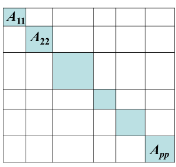
\includegraphics[width=0.8\textwidth]{./figures/figure2.png} 
\end{figure}
\begin{itemize}
\item {\color{blue}分块Jacobi迭代}$$
A_{i i} \boldsymbol{x}_{i}^{(k+1)}=\boldsymbol{b}_{i}-\sum_{j=1, j \neq i}^{p} A_{i j} \boldsymbol{x}_{j}^{(k)}, \quad i=1,2, \ldots, p
$$
\item {\color{blue}分块Gauss-seidel迭代}$$
A_{i i} \boldsymbol{x}_{i}^{(k+1)}=\boldsymbol{b}_{i}-\sum_{j=1}^{i-1} A_{i j} \boldsymbol{x}_{j}^{(k+1)}-\sum_{j=i+1}^{p} A_{i j} \boldsymbol{x}_{j}^{(k)}, \quad i=1,2, \ldots, p
$$
\item {\color{blue}分块SOR迭代}$$
\begin{array}{c}{\boldsymbol{x}_{i}^{(k+1)}=(1-\omega) \boldsymbol{x}_{i}^{(k)}+\omega A_{i i}^{-1}\left(\boldsymbol{b}_{i}-\sum_{j=1}^{i-1} A_{i j} \boldsymbol{x}_{j}^{(k+1)}-\sum_{j=i+1}^{p} A_{i j} \boldsymbol{x}_{j}^{(k)}\right)} \\ {i=1,2, \ldots, p}\end{array}
$$
\end{itemize}
%\newpage
\section{\color{blue}收敛性分析}
%\newpage
\subsection{定常迭代方法的收敛性}




































































\cite{tam19912d}
\bibliography{ref}
\end{document}
